\documentclass[parskip=half]{scrartcl}
	
\usepackage[english]{babel}
\usepackage[latin1]{inputenc}
\usepackage{enumerate} % til \begin{enumerate}[(i)]
\usepackage{enumitem} % til at styre lister globalt
\usepackage{latexsym} % symboler
\usepackage{amsthm} % til thm osv
\usepackage{amssymb} % flere symbloer
\usepackage{bm} % bold math symbols
\usepackage{amsmath} % til pmatrix
\usepackage[hyphens]{url} %til \url med bindestreger
%\PassOptionsToPackage{hyphens}{url}\usepackage{hyperref}
\usepackage[pdftex]{graphicx}	
\usepackage{scrlayer-scrpage} % page setup

\usepackage[cache=false]{minted} % for source code
\usepackage{xcolor}
%set page header
\chead{FYS-STK4155 --- project 1}


% List will number things using (a), (b), ...
\setenumerate[1]{label={(\alph*)}} % Global setting

% Title setup
\title{Report for project 1}
\date{\today}
\author{Adam P W S{\o}rensen}

%%%%%%%%%%%%
% make chi subscripts low enough
% from http://tex.stackexchange.com/questions/191551/greek-chis-subscript-expressions-how-to-make-it-smaller-or-offset-lower
\let\latexchi\chi
\makeatletter
\renewcommand\chi{\@ifnextchar_\sub@chi\latexchi}
\newcommand{\sub@chi}[2]{% #1 is _, #2 is the subscript
  \@ifnextchar^{\subsup@chi{#2}}{\latexchi^{}_{#2}}%
}
\newcommand{\subsup@chi}[3]{% #1 is the subscript, #2 is ^, #3 is the superscript
  \latexchi_{#1}^{#3}%
}
\makeatother

\newcommand{\setof}[2]{\left\{ #1 \; \middle\vert \; #2 \right\}}

\DeclareMathOperator{\cspan}{\overline{span}}

% Theorem opsætning
\newtheorem{theorem}{Theorem}[section]
\newtheorem*{theorem*}{Theorem}
\newtheorem{lemma}[theorem]{Lemma}
\newtheorem{corollary}[theorem]{Corollary}
\newtheorem{proposition}[theorem]{Proposition}
\newtheorem{example}[theorem]{Example}
\newtheorem{conjecture}[theorem]{Conjecture}
\theoremstyle{definition}
\newtheorem{definition}[theorem]{Definition}
\newtheorem{assumption}[theorem]{Standing Assumption}
\newtheorem*{assumption*}{Standing Assumption}
\theoremstyle{remark}
\newtheorem{remark}[theorem]{Remark}
\newtheorem{notation}[theorem]{Notation}

%%%%%%%%%%%%
% notation short cuts
\newcommand{\vect}[1]{{\bm{#1}}}
\newcommand{\funcname}[1]{{\color{blue}{\texttt{#1}}}}
\newcommand{\varname}[1]{\texttt{#1}}
%%%%%%%%%%%%
% bb letters
\newcommand{\C}{\mathbb{C}}
\newcommand{\E}{\mathbb{E}}
\newcommand{\N}{\mathbb{N}}
\newcommand{\Q}{\mathbb{Q}}
\newcommand{\R}{\mathbb{R}}
\newcommand{\Z}{\mathbb{Z}}
% cal letters
\newcommand{\A}{\mathcal{A}}
\newcommand{\B}{\mathcal{B}}
\newcommand{\D}{\mathcal{D}}
\newcommand{\cL}{\mathcal{L}}
\newcommand{\M}{\mathcal{M}}
\newcommand{\cZ}{\mathcal{Z}}
% frak letters
\newcommand{\fA}{\mathfrak{A}}


%%%%%%%%%%%%%%
\begin{document}
%%%%%%%%%%%%%%

\maketitle

\begin{abstract}
In this project we used three different linear regression methods to approximate the Franke Function and some real world terrain data. 
The methods we use are the Ordinary Least Square, Ridge, and Lasso regression. 
For each we use a 10-fold cross validation to pick the best model and then we preform statistical tests to ascertain the validity of our models. 
None of them are particularly good. 
\end{abstract}


\section{Introduction}

This project is concerned with the following problem: Suppose we know the values of a function $f$ on a set of points $\{x_1, x_2, \ldots, x_n\}$, can we then predict $f(x)$ for any $x$?
In full generality this is plainly impossible (though see \cite{ht:choice}).
But if we allow ourselves to believe that the function $f$ is not too erratic, then we can certainly try to notice a pattern and use that for our predictions.
Like in an IQ test.
In fact we would also like to find a pattern even if we do not know $f(x_i)$ exactly, but only with some small noise thrown in.
This corresponds more closely to a real world measurement scenario. 

Linear Regression methods are a mathematical rigorous way of noticing these types of patterns.
The methods produce a so-called parameter vector from the know values of $f$ and then produce a prediction functions that is linear in this parameter vector, and not in the inputs $x$. 
A typical usage is to try to find a polynomial approximation of $f$. 
If we have $n$ data points $\{x_1, x_2, \ldots, x_n\}$ and we know the function values $f(x_i)$ one can perfectly fit a $n-1$ degree polynomial to this data.
This will usually be the wrong approach. 
Suppose we measure the following. 

\begin{center}
\begin{tabular}{l|cccc}
x & 1 & 2 & 3 & 4\\
\hline
f(x) & 1.1 & 1.9 & 3.1 & 3.9
\end{tabular} 
\end{center} 

Any sane person would predict that $f(5)$ ought to be almost $5$ (they might even predict that it is $5.1$). 
Figure 1 shows a what happens when we try to predict from this using a basic linear regression method to get either a first or third degree polynomial.

\begin{figure}[H]
\caption{An example of over fitting.}
\centering
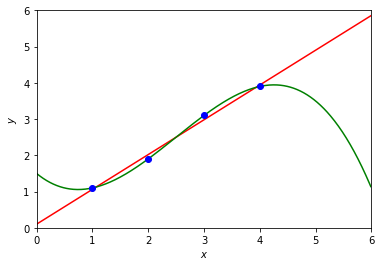
\includegraphics[scale=0.5]{overfitting.png}
\end{figure}

The green line shows the third degree polynomial, the red line is the first degree polynomial and the blue dots are the observations. 
We see that the third degree polynomial predicts that $f(5) \approx 3.5$. 

To avoid this type of problem one has to validate the model used.
A simple test that would have worked here is to try to predict using only some of the observation, and then test against the remaining observations.
In general we use sophisticated test, in such test is called cross validation which we will discuss below.   

In this report we will discuss three specific linear regression methods: Ordinary Least Squares, Ridge, and Lasso regression.
We will talk about the weakness and strengths of each one. 
We will apply them to the so-called Franke function and some real world terrain data and discuss how successful they are, as determined by statistical tests.
It will unfortunately transpire that neither of our methods are particularly good for predicting the behaviour of Franke function or the terrain data.
 
All reference to code refer to the jupyter notebook \texttt{Projekt 1.ipynb}.
The report is structured as follows. 
In Section \ref{sec:lrm} we will introduce, more rigorously, linear regression and discuss the three specific methods we use. 
We will touch on their theory and how I have coded them.
In Section \ref{sec:selection} we turn our attention to model selection and validation, looking at cross validation and the bias and variance of a model. 
Again there is brief discussion of the theory and comments on the implementation. 
In sections \ref{sec:franke} and \ref{sec:terrain} we look at how our models work on the Franke function and the terrain data. 
Finally in Section \ref{sec:conclusion} we summarize our findings. 

\section{Linear Regression Methods} \label{sec:lrm}
 
Broadly speaking the idea of linear regression is as follows.
We are given $N$ data points each represented by a row vector $\vect{x_i}$ of some size $p$ and the corresponding real measurements $z_1, z_2, \ldots z_N$. 
Then we try to find a column vector $\vect{\beta}$ such that 
\[
	\begin{pmatrix}
		\vect{x_1} \\
		\vect{x_2} \\
		\vdots \\
		\vect{x_n}
	\end{pmatrix} \vect{\beta}
	\approx
	\begin{pmatrix} z_1 \\ z_2 \\ \vdots \\ z_n \end{pmatrix}.	
\]

The goal is choose $\vect{\beta}$ such that the approximate equality holds as best as possible. 
Exactly how we measure what it means for two vectors to be approximately equal will define the different regression methods. 

In our case we are interested in finding a polynomial that approximates a function $f$ of two variables.
When we want a polynomial of degree $d$ we will first find $N$ points in the plane $(x_1, y_1), (x_2, y_2), \ldots (x_N, y_N)$ and record the values $z_1 = f(x_1, y_1), z_2 = f(x_2, y_2) \ldots z_N = f(x_N, y_N)$.
The data points will not only be the pairs $(x_i, y_i)$ but instead the row vectors 
\[
	\vect{x_i} = \begin{pmatrix} 1 & x_i & y_i & x_i^2 & x_i y_i & y_i^2 & \cdots & y_i^d \end{pmatrix},
\]
containing all expressions $x_i^k y_i^l$ with for $k,l$ non-negative integers with $k+l \leq d$. 
To ease notation we put 
\[
 X = \begin{pmatrix} \vect{x_1} \\ \vect{x_2} \\ \vdots \\ \vect{x_N} \end{pmatrix},
 \quad \text{ and } \quad
 \vect{z} = \begin{pmatrix} z_1 \\ z_2 \\ \vdots \\ z_N \end{pmatrix}. 	
\]
The goal is then to find $\vect{\beta}$ such that 
\begin{equation} \label{eq:linreg}
	X \vect{\beta} \approx \vect{z}.
\end{equation}
Given such a $\vect{\beta}$ we can then \emph{predict}, or perhaps more accurately estimate, the value of $f$ at a given point $(x,y)$ by computing 
\begin{equation} \label{eq:linregpredict}
	\begin{pmatrix} 1 & x & y & x^2 & xy & y^2 & \cdots & y^d \end{pmatrix} \vect{\beta} 
	=
	\beta_1  + \beta_2 x + \beta_3 y  + \beta_4 x^2 + \cdots.
\end{equation}
   
The expression on the right hand side is our polynomial approximation of $f$. 

We now consider three kinds of linear regression: Ordinary Least Square, Ridge and Lasso. 
Below we briefly discuss the theory of each and how they were implemented in the code.
It is all implemented in the third code block in the jupyter notebook, and in the fourth it is tested against the functionalities provided by sci-kit learn. 

\subsection{Ordinary Least Square Regression}

In the Ordinary Least Square method (described in Section 3.2 of \cite{htf:esl}) we measure the approximate equality in equation (\ref{eq:linreg}) in 2-norm. 
That is we are looking for a $\vect{\beta}$ the minimizes 
\[
	\| X \vect{\beta} - \vect{z} \|_2,
\] 
where $\|\cdot\|_2$ denotes the 2-norm, i.e. the usual euclidean distance.
From equation (3.6) in \cite{htf:esl} we see that this is achieved  by setting 
\[
	\vect{\beta} = (X^T X)^{-1}X^T \vect{z}.
\] 

In the code this is implemented by $2$ classes and one ancillary function. 
The function \funcname{polymatrix} takes a matrix with two columns, called $\vect{x}$ and $\vect{y}$, and and a natural number d, it produces the following matrix 
\[
	\begin{pmatrix}
	 \vect{1} & \vect{x} & \vect{y} & \vect{x}^2 & \vect{x} \vect{y} & \vect{y}^2 & \cdots & \vect{y}^d 
	\end{pmatrix},
\]
where all multiplications are done pointwise.
In other words \funcname{polymatrix} constructs the matrix we called $X$ above.
To implement \funcname{polymatrix} we first note that picking non-negative $k,l$ such that $0 < k+l \leq d$ is the same as picking $k-i,i$ such that $1 \leq k \leq d$ and $0 \leq i \leq k$. 
Now \funcname{polymatrix} first computes a list where each entry is a column vector of the form $\vect{x}^{k-i} \vect{y}^{i}$, and then use \varname{np.hstack} to combine them and a column vector of ones into a single matrix. 

The class \funcname{myOLS} has a single variable \varname{beta} and two functions \funcname{train} and \funcname{predict}. 
The function \funcname{train} just uses numpy to implement equation (3.6) in \cite{htf:esl}, simlarly \funcname{predict} implements the predict equation (\ref{eq:linregpredict}) using numpy.
The whole reason for this class is just to make the next one have cleaner code.

The class \funcname{polynomialOLS} is what we use to do our OLS regression. 
When initiating an instance of this class, one has to give the degree of the polynomial we want to approximate by. 
The functions \funcname{train} and \funcname{predict} both expect a matrix \varname{XY} with two columns, each row having a coordinate pair $x,y$, in addition \funcname{train} needs a column vector $\vect{z}$ of real function values. 
They both first use \funcname{polymatrix} to build the right matrix, as discussed above, and the simply call the \funcname{train} and \funcname{predict} from \funcname{myOLS}.
The design choice of making the \funcname{train} and \funcname{predict} functions take care of transforming the input from $x,y$ pairs to the polynomial matrix, was to make later code more readable by avoiding having to make the transformation before each call. 
In addition \funcname{polynomialOLS} has function to return the computed vector $\vect{\beta}$, a function to print some info about the model, and a function I use for plotting.
I suspect the latter is quite unnecessary, and could be removed if I were better at using numpy's vectorize functionality. 

\subsection{Ridge Regression}  

The theory for Ridge regression is described in Section 3.4.1 of \cite{htf:esl}. 
For ridge regression we need a parameter $\lambda > 0$ in addition to the input data matrix $X$ and a true value vector $\vect{z}$.
The method is similar to OLS, but the inclusion of $\lambda$ is used to reduce the variance of the computed $\vect{\beta}$ which in OLS can change a lot with small changes of inputs.    
When choosing $\beta$ we again want to minimize the 2-norm of $\vect{z} - X\vect{\beta}$ but at the same time also the expression 
\[
	\lambda \sum_{i=1}^p \beta_i^2 \quad \text{where} \quad  \vect{\beta} = \begin{pmatrix}\beta_0 \\ \beta_1 \\ \vdots \\ \beta_p \end{pmatrix}.	     
\]
Note that $\beta_0$ is not included, that is we don't penalize the constant term of our polynomial. 
Like for the OLS case there is an explicit formula for $\vect{\beta}$.
For this, we do not include the column of $1$'s in the matrix $X$ and we assume that each column of $X$ has been centered (i.e. has mean $0$), then by equation (3.44) in \cite{htf:esl}:
\begin{equation} \label{eq:ridgebeta}
	\vect{\beta} = \left(X^T X + \lambda I \right)^{-1} X^T y. 
\end{equation}
This only gives the $\beta_1, \beta_2, \ldots, \beta_p$. 
We set $\beta_0$ to be the mean of $\vect{z}$.

If we do not assume that $X$ is centered we let $\bar{x}_i$ be the mean of the $i$'th column of $X$, and replace $X$ with the matrix $(x_{ij} - \bar{x}_j)_{i,j}$. 
Following programming conventions we will still call this matrix $X$.
We still use equation (\ref{eq:ridgebeta}) to compute the $\beta_1, \beta_2 \ldots, \beta_p$, however we put
\begin{equation} \label{eq:ridgeintercept}
	\beta_0 = E(\vect{z}) - \begin{pmatrix} \bar{x}_1 & \bar{x}_2 & \cdots & \bar{x}_p \end{pmatrix} \begin{pmatrix} \beta_1 \\ \beta_2 \\ \vdots \\ \beta_p \end{pmatrix},
\end{equation}
where $E(\vect{z})$ denote the mean of $\vect{z}$. 
The term we subtract can be thought of as retransforming the intercept out of the assumption the columns are centered. 

In the code the class \funcname{polynomialRidge} implements Ridge regression. 
To initiate an instance of this class one needs to give the degree of the polynomial we want to approximate by, and the parameter $\lambda$. 
(\funcname{lambda} has its own python meaning so we cannot use that for the parameter).
Again the most interesting functions are \funcname{train} and \funcname{predict}. 
As in the OLS case we use \funcname{polymatrix} to go from two columns of x's and y's too the all the terms of polynomial. 
The heavy duty of centering and uncentering is done in \funcname{train}, which just uses numpy to implement the maths described above. 
Because of that $\funcname{predict}$ is just as straight forward as it was in the OLS case.
In both \funcname{train} and \funcname{predict} we must delete the column of $1$'s coming from \funcname{polymatrix} as the intercept is treated different from all other $\beta$ parameters. 
As for OLS we also have some extra functions that are used later to print and extract parameters. 

\subsection{Lasso Regression} \label{sec:selection}

Lasso regression is similar to Ridge regression in that it uses a parameter $\lambda$ to lessen the variance of the computed $\beta_i$, however unlike Ridge and OLS it is much more likely to set a given $\beta_i$ equal to $0$. 
We will see this a lot later. 
The theory of Lasso regression is in Section 3.4.2 of \cite{htf:esl}. 
Like in Ridge regression we try to minimize not only $\|\vect{z} - X \vect{\beta}\|_2$ but at the same time also an extra term, which in the Lasso case is  
\[
	\lambda \sum_{i=1}^p |\beta_i|.
\] 
So it is the $1$-norm of $\vect{\beta}$ (without its first row) instead of the $2$-norm in Ridge. 
Here there is no closed form expression for $\vect{\beta}$.

The implementation of Lasso regression is in the class \funcname{polynomialLasso}. 
We use sci-kit learns Lasso regression functionality and \funcname{polynomialLasso} just acts as a wrapper that takes care to transform the input appropriately. 
It is in all respects the same as how \funcname{polynomialOLS} used the class \funcname{myOLS}.

\section{Model Selection and Verification}

\subsection{Cross Validation}

To choose between different models I used cross validation, implemented in the fifth code block of the jupyter notebook. 
I build the code on the theory described in Section 7.10.1 of \cite{htf:esl}. 
In the optimal situation where we have easy access to lots of data, we would split our data in to three parts, one part for training or models, one part for used to decide between models, and then a final part to test the reliability of our chosen model. 
We are actually in this situation, but will pretend we are not. 

The purpose of cross validation is to not keep a partition of the data specifically for validation, and instead use the training data for validation. 
It works as follows.
Suppose we have a model $M$ and our training data are data points $\{\vect{x}_i\}_{i=1}^N$ with corresponding true values $\{z_i\}_{i=1}^N$.
We fix a natural number $k$, which is the number of so-called folds we will use.  
Then we partition $\{1,2,\ldots, N\}$ into $k$ almost equally big sets $A_1, A_2, \ldots, A_k$.
In symbols 
\[
	\{1,2,\ldots, N\} = \bigsqcup_{j=1}^k A_j.
\]  
For each $j$ we train our model $M$ on $\{1,2,\ldots, N\} \setminus A_j$ and call the corresponding prediction function $f_j$. 
Now we estimate the square error this model will lead to on an unseen data point, denoted $cv$, by 
\[
	cv = \frac{1}{N} \sum_{j=1}^k \sum_{i \in A_j} (f_j(\vect{x}_i) - z_i)^2. 
\]
Note that the prediction of $\vect{x}_i$ is done by a model not trained on $\vect{x}_i$.
In case $k$ even divides $N$ so that all the $A_j$ are of size $N/k$ we can write this as 
\[
	cv = \frac{1}{k} \sum_{j=1}^k \left[ \frac{1}{|A_j|} \sum_{i \in A_j} (f_j(\vect{x}_i) - z_i)^2 \right].
\]
Here the terms enclosed in $[\cdot]$ is just the mean squared error the model $M$ makes when trained on $\{1,2,\ldots, N\} \setminus A_j$ and then tested against $A_j$.
So we can think of the cross validation error estimate as an average of mean squared errors. 

Obviously different choices of $k$ will lead to different estimated errors. 
So the choice of $k$ seems more art than science, but apparently $k=10$ is an established best practise.

In the code I have implemented a function \funcname{cross{\_}validation} to do cross validation. 
It takes 4 arguments, the number of folds \varname{k}, a two column matrix \varname{XY} of input data, a column vector \varname{z} or true values, and a model \varname{model} which has \funcname{train} and \funcname{predict} functions. 
Clearly these functions should work on the data points and true values. 
The idea is to use the regression methods I have implemented above as one of the models. 

For the implementation we first record the length of the columns, $N$ say, in \varname{XY} and then use numpy functions to partition $\{1,2,\ldots, N\}$ into \varname{k} sets. 
We loop over the folds and use an indexing mask to pick out all the data not in the current fold, train the model on it, and record the squared differences between prediction from the current fold and the real data. 
Finally we return the average of all these squared errors. 

Numpy contains a function called \funcname{cross\_ val\_ score} that I would have liked to compare my code to.
However I couldn't get it to play well with my regression methods.
The documentation for \funcname{cross\_val\_score} (\url{http://scikit-learn.org/stable/modules/generated/sklearn.model_selection.cross_val_score.html}) says the estimator, what I called model, should implement a \funcname{fit} function. 
But even if rename my \funcname{train} to \funcname{fit}, or indeed just add the line \mintinline{python}{self.fit = self.train} to the \funcname{\_\_init\_\_} of my classes, I still get errors asking for more functions to be implemented. 
I chose not to track through the numpy documentation to figure out what exactly I needed to implement. 
Instead, I am contended to note the the predicted errors seem somewhat close to the actual errors we get when testing against unseen data. 

\subsection{Verification}

Once a model is chosen, we want to see how stable and accurate it is. 
To this end in the sixth code block of the jupyter notebook I have done basic implementations of mean squared error functions, $R^2$ score, and variance of the entries of vector. 
There are formulas for these which I just translated to numpy. 
In the seventh code block they are tested against the native numpy functions and give the same results.

In the eighth code block I implement a function \funcname{BV\_estimate} to record the bias and variance of our model, I also implement \funcname{beta\_variance} to record the variance of the $\beta_i$'s.   
Both are based on the ideas of cross fold validation. 
For \funcname{BV\_estimate} we proceed similarly to cross fold validation and partition $\{1,2,\ldots, N\}$, but this time into $k+1$ folds $\{A_j\}_{j=1}^{k+1}$. 
We now successively train the on each of $\{1,2,\ldots N\} \setminus (A_j \cup A_{k+1})$ to get a prediction function $f_j$ which is tested against $A_{k+1}$. 
This way we get multiple predictions for each point in $A_{k+1}$ and so can compute the models bias and variance as
\[
	\text{bias}^2 = \frac{1}{|A_{k+1}|} \sum_{i \in A_{k+1}} \left[ \frac{1}{k} \sum_{j=1}^{k} (f_j(\vect{x}_i) - z_i) \right]
\]	
and 
\[
	\text{variance} = \frac{1}{|A_{k+1}|} \sum_{i \in A_{k+1}} \left[ \operatorname{Var}(f_j(\vect{x}_i)) \right],
\]
where the $\operatorname{Var}(f_j(\vect{x}_{i}))$ is taken as $j$ varies and $i$ is kept fixed. 
The theory of this is described in Section 7.3 of \cite{htf:esl}, but the implementation is mostly based on the piazza note on Bias and Variance of a model.

The function \funcname{beta\_variance} is again build in a way very similar to \funcname{cross\_validation}. 
This time instead of recording prediction errors I record the coefficient vector $\vect{\beta}_j$ of each training session, and then compute the variance of each entry. 

A reasonable critic of both methods is that I should perhaps repeat the k-fold process a number of times to get more $\vect{\beta}$s or point predictions to get more accurate variances.
However, if 10 folds works for cross prediction it probably works fine for these.

\section{Results on the Franke Function (parts a,b,c)} \label{sec:franke}

The code blocks 9-17 looks at the Franke Function and the different linear regression methods. 
In block 9 the data is setup, I pick 1000 pairs $(x,y)$ in $[0,1]^2$ and record their real values with a little added noise. 
I used cross validation for each regression method and picked the model that gave the smallest predicted error.

\begin{tabular}{l|ccc}
Regression Method & Polynomial degree & lambda parameter & Predicted error \\ 
\hline
\hline 
OLS & 5 &  & 0.044361 \\ 
Ridge & 5 & 0.1 & 0.049839 \\ 
Lasso & 4 & 0.1 & 0.124234
\end{tabular} 

For each of the best methods I computed the actual mean squared error and $R^2$ score against unseen data. 
I also found the model vaiance and bias.

\begin{tabular}{l|cccc}
Regression Method & Mean squared error & $R^2$ & bias$^2$ & model variance  \\ 
\hline
\hline 
OLS &  0.046539 & 0.636927 & 0.043213 & 0.000132 \\ 
Ridge & 0.058986 & 0.539831 & 0.054887 & 0.000056 \\ 
Lasso & 0.130758 & -0.020091 & 0.128723 & 0.000007
\end{tabular} 

On the positive side, we note that the actual mean squared errors are somewhat close to the predicted values.
We also see that as expected the bias of OLS is smallest, then Ridge and then Lasso, and the variances go the other way.    
Other than that, there is not a lot of positive things to say about these models. 
They have abysmal $R^2$ scores.
In particular I am puzzled by the negative score for the Lasso regression, if one looks at the model, we will see that all parameters except the intercept are zero. 
However, an $R^2$ score of $0$ is suppose to indicate that your model is no better then a hyperplane. 
So the Lasso model I found manages to be a bad hyperplane model.  

Let us now take closer look at coefficients (see code blocks 54, 57, and 66).
The first thing that springs out, is that as noted that all the Lasso coefficients, except the intercept, are $0$ and that they have no variance. 
There is a small variance on the intercept, but it is of the order of $10^{-5}$. 
Thus the Lasso model is very confident in its poor prediction. 
That all the parameters are set to zero is a feature of the Lasso model, but in this case it works against it. 

The next thing to notice is how big some of the coefficients of the OLS regression are.
For instance $\beta_3$, which corresponds to the $x^2$ term is $-28.83003238$, and there is a variance on it of $8.30320758$.
So we get a $95\%$ confidence interval (rounded off) for $\beta_4$ of 
\[
	[-28.83 - 2 \times 8.30; -28.83 + 2 \times 8.30] = [-45.43; -12.23].  
\]
So I am $95\%$ sure the real value of $\beta_d$ is between $-45$ and $-12$.
Which I read to mean that the computation is almost meaningless. 

Turning to Ridge regression we see much smaller coefficients and much smaller variance of the $\beta_i$. 
Looking again at $\beta_3$, the $x^2$ term, here it is $-1.5575589$ with a variance of $0.00327892$, which gives a $95\%$ confidence interval of $\beta_3$ of 
\[
	[-1.56411674; -1.55100106].
\]
The variance for all the $\beta_i$ are similarly small so we will get similar confidence intervals. 

Looking at all the data, it seems that the Ridge regression giving a fifth degree polynomial with a $\lambda$ parameter of $0.1$ gives the best model. 
While it has a worse $R^2$ score than the OLS model, its much more stable behaviour gives it the nudge. 

\section{Results for Terrain Data} \label{sec:terrain}

For the terrain data I chose a picturesque mountain range just outside of Sydney called the Blue Mountains. 
I again used cross validation to select the model with the smallest predicted error (code block 68), and I got Ridge regression for a third degree polynomial with a $\lambda$ parameter of $0.5$.
Running statistical tests as above, I got the following.

\begin{tabular}{l|cccc}
Regression method & mean squared error & $R^2$ & bias$^2$ & model variance  \\ 
\hline
\hline 
Ridge & 27383.656382 & 0.767798 & 24636.566560 & 5.116623 \\ 
\end{tabular} 

The first thing to note is the enormous mean squared error. 
This number was expected to be bigger than for the Franke Function, from the simple fact that the terrain data function takes values in a much bigger range. 
I also note that we have an almost respectable $R^2$ score of approximately $0.77$, nothing impressive but notably better than for the Franke Function. 
There is very little variance on the $\beta_i$'s except for the intercept, where the variance is $14.2955179$, leading to a confidence interval on $\beta_0$ of 
\[
	[745.8323202; 803.0143918]
\]
For a final test, I plotted a 500 by 500 corner of the map, and the same corner as predicted by the model in code block 76. 
Looking at it, we can see that the model picks up the very bright spot in the lower left corner and sort of picks up the dark lines running along the X-axis around Y-coordinate 100--200. 
In a way the predicted map looks like a very blurry version of the real map. 

\section{Conclusion} \label{sec:conclusion}

From the modelling of the Franke function and the terrain date, we see that the linear regression methods acts as the theory predicts.
The Ridge and Lasso regressions are more stable than the Ordinary Least Squares regression and Lasso is much more likely to set a given $\beta_i$ to $0$. 
None of the linear regression methods are particularly well suited for these particular problems. 
Hence other methods are needed if we want useful predictions. 

%%%%%%%%%%%%%%
%Bibliography
\newpage
\bibliographystyle{apalike}
\bibliography{refs}	% expects file "refs.bib"
%%%%%%%%%%%%%%


\end{document}